

\tikzset{every picture/.style={line width=0.75pt}} %set default line width to 0.75pt        

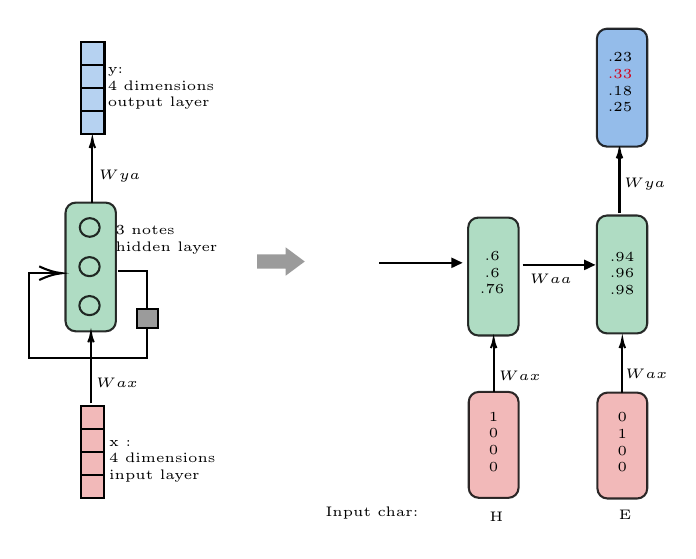
\begin{tikzpicture}[x=0.75pt,y=0.75pt,yscale=-1,xscale=1]
%uncomment if require: \path (0,300); %set diagram left start at 0, and has height of 300

%Rounded Rect [id:dp5767801512845814] 
\draw  [color={rgb, 255:red, 0; green, 0; blue, 0 }  ,draw opacity=0.82 ][fill={rgb, 255:red, 78; green, 178; blue, 121 }  ,fill opacity=0.45 ][line width=0.75]  (117.57,131.31) .. controls (117.57,128.63) and (119.74,126.46) .. (122.42,126.46) -- (136.98,126.46) .. controls (139.66,126.46) and (141.83,128.63) .. (141.83,131.31) -- (141.83,183.6) .. controls (141.83,186.28) and (139.66,188.46) .. (136.98,188.46) -- (122.42,188.46) .. controls (119.74,188.46) and (117.57,186.28) .. (117.57,183.6) -- cycle ;
%Straight Lines [id:da08198893479819136] 
\draw    (323.83,217.67) -- (323.83,194.17) ;
\draw [shift={(323.83,192.17)}, rotate = 450] [color={rgb, 255:red, 0; green, 0; blue, 0 }  ][line width=0.75]    (4.37,-1.32) .. controls (2.78,-0.56) and (1.32,-0.12) .. (0,0) .. controls (1.32,0.12) and (2.78,0.56) .. (4.37,1.32)   ;
%Straight Lines [id:da27259750014998585] 
\draw    (337.83,156.46) -- (369.83,156.46) ;
\draw [shift={(372.83,156.46)}, rotate = 180] [fill={rgb, 255:red, 0; green, 0; blue, 0 }  ][line width=0.08]  [draw opacity=0] (5.36,-2.57) -- (0,0) -- (5.36,2.57) -- cycle    ;
%Straight Lines [id:da14030301096924913] 
\draw    (384.48,131.46) -- (384.48,102.75) ;
\draw [shift={(384.48,100.75)}, rotate = 450] [color={rgb, 255:red, 0; green, 0; blue, 0 }  ][line width=0.75]    (4.37,-1.32) .. controls (2.78,-0.56) and (1.32,-0.12) .. (0,0) .. controls (1.32,0.12) and (2.78,0.56) .. (4.37,1.32)   ;
%Straight Lines [id:da5186597746729542] 
\draw    (268.83,155.46) -- (305.83,155.46) ;
\draw [shift={(308.83,155.46)}, rotate = 180] [fill={rgb, 255:red, 0; green, 0; blue, 0 }  ][line width=0.08]  [draw opacity=0] (5.36,-2.57) -- (0,0) -- (5.36,2.57) -- cycle    ;
%Right Arrow [id:dp4588186786561803] 
\draw  [draw opacity=0][fill={rgb, 255:red, 155; green, 155; blue, 155 }  ,fill opacity=1 ] (209.83,151.42) -- (223.63,151.42) -- (223.63,148) -- (232.83,154.83) -- (223.63,161.67) -- (223.63,158.25) -- (209.83,158.25) -- cycle ;
%Straight Lines [id:da49006821221672503] 
% \draw    (398.83,156.46) -- (432.83,156.46) ;
% \draw [shift={(435.83,156.46)}, rotate = 180] [fill={rgb, 255:red, 0; green, 0; blue, 0 }  ][line width=0.08]  [draw opacity=0] (5.36,-2.57) -- (0,0) -- (5.36,2.57) -- cycle    ;
%Shape: Ellipse [id:dp18804427153778946] 
\draw  [color={rgb, 255:red, 0; green, 0; blue, 0 }  ,draw opacity=0.82 ] (124.44,138.43) .. controls (124.44,135.95) and (126.58,133.93) .. (129.23,133.93) .. controls (131.88,133.93) and (134.02,135.95) .. (134.02,138.43) .. controls (134.02,140.91) and (131.88,142.92) .. (129.23,142.92) .. controls (126.58,142.92) and (124.44,140.91) .. (124.44,138.43) -- cycle ;
%Shape: Ellipse [id:dp672728185189052] 
\draw  [color={rgb, 255:red, 0; green, 0; blue, 0 }  ,draw opacity=0.82 ] (124.22,176.07) .. controls (124.22,173.53) and (126.41,171.47) .. (129.12,171.47) .. controls (131.83,171.47) and (134.02,173.53) .. (134.02,176.07) .. controls (134.02,178.61) and (131.83,180.67) .. (129.12,180.67) .. controls (126.41,180.67) and (124.22,178.61) .. (124.22,176.07) -- cycle ;
%Shape: Ellipse [id:dp22457931655016228] 
\draw  [color={rgb, 255:red, 0; green, 0; blue, 0 }  ,draw opacity=0.82 ] (124.22,157.3) .. controls (124.22,154.76) and (126.41,152.7) .. (129.12,152.7) .. controls (131.83,152.7) and (134.02,154.76) .. (134.02,157.3) .. controls (134.02,159.84) and (131.83,161.9) .. (129.12,161.9) .. controls (126.41,161.9) and (124.22,159.84) .. (124.22,157.3) -- cycle ;
%Shape: Rectangle [id:dp3603601739458042] 
\draw  [fill={rgb, 255:red, 234; green, 141; blue, 141 }  ,fill opacity=0.61 ] (124.9,224.38) -- (136.12,224.38) -- (136.12,235.47) -- (124.9,235.47) -- cycle ;
%Shape: Rectangle [id:dp3229189908551803] 
\draw  [fill={rgb, 255:red, 234; green, 141; blue, 141 }  ,fill opacity=0.61 ] (124.9,235.47) -- (136.12,235.47) -- (136.12,246.56) -- (124.9,246.56) -- cycle ;
%Shape: Rectangle [id:dp21435953126093987] 
\draw  [fill={rgb, 255:red, 234; green, 141; blue, 141 }  ,fill opacity=0.61 ] (124.9,246.56) -- (136.12,246.56) -- (136.12,257.64) -- (124.9,257.64) -- cycle ;
%Shape: Rectangle [id:dp23717670155716364] 
\draw  [fill={rgb, 255:red, 234; green, 141; blue, 141 }  ,fill opacity=0.61 ] (124.9,257.64) -- (136.12,257.64) -- (136.12,268.73) -- (124.9,268.73) -- cycle ;

%Shape: Rectangle [id:dp5297698591025225] 
\draw  [fill={rgb, 255:red, 148; green, 188; blue, 234 }  ,fill opacity=0.68 ] (125.11,49.12) -- (136.33,49.12) -- (136.33,60.21) -- (125.11,60.21) -- cycle ;
%Shape: Rectangle [id:dp38660215409167686] 
\draw  [fill={rgb, 255:red, 148; green, 188; blue, 234 }  ,fill opacity=0.68 ] (125.11,60.21) -- (136.33,60.21) -- (136.33,71.3) -- (125.11,71.3) -- cycle ;
%Shape: Rectangle [id:dp69064370761254] 
\draw  [fill={rgb, 255:red, 148; green, 188; blue, 234 }  ,fill opacity=0.68 ] (125.11,71.3) -- (136.33,71.3) -- (136.33,82.39) -- (125.11,82.39) -- cycle ;
%Shape: Rectangle [id:dp2596136729141916] 
\draw  [fill={rgb, 255:red, 148; green, 188; blue, 234 }  ,fill opacity=0.68 ] (125.11,82.39) -- (136.33,82.39) -- (136.33,93.48) -- (125.11,93.48) -- cycle ;

%Straight Lines [id:da21936148645185471] 
\draw    (129.83,223.17) -- (129.83,191.38) ;
\draw [shift={(129.83,189.38)}, rotate = 450] [color={rgb, 255:red, 0; green, 0; blue, 0 }  ][line width=0.75]    (4.37,-1.32) .. controls (2.78,-0.56) and (1.32,-0.12) .. (0,0) .. controls (1.32,0.12) and (2.78,0.56) .. (4.37,1.32)   ;
%Straight Lines [id:da5720693198246461] 
\draw    (130.48,126.46) -- (130.48,97.75) ;
\draw [shift={(130.48,95.75)}, rotate = 450] [color={rgb, 255:red, 0; green, 0; blue, 0 }  ][line width=0.75]    (4.37,-1.32) .. controls (2.78,-0.56) and (1.32,-0.12) .. (0,0) .. controls (1.32,0.12) and (2.78,0.56) .. (4.37,1.32)   ;
%Straight Lines [id:da45318748010738064] 
\draw    (142.83,159.46) -- (156.83,159.46) -- (156.83,201.46) -- (99.83,201.46) -- (99.83,160.46) -- (113.83,160.46) ;
\draw [shift={(115.83,160.46)}, rotate = 180] [color={rgb, 255:red, 0; green, 0; blue, 0 }  ][line width=0.75]    (10.93,-3.29) .. controls (6.95,-1.4) and (3.31,-0.3) .. (0,0) .. controls (3.31,0.3) and (6.95,1.4) .. (10.93,3.29)   ;
%Shape: Rectangle [id:dp46321775555410516] 
\draw  [fill={rgb, 255:red, 155; green, 155; blue, 155 }  ,fill opacity=1 ] (151.83,177.79) -- (162.25,177.79) -- (162.25,186.96) -- (151.83,186.96) -- cycle ;
%Rounded Rect [id:dp9185519263132114] 
\draw  [color={rgb, 255:red, 0; green, 0; blue, 0 }  ,draw opacity=0.82 ][fill={rgb, 255:red, 78; green, 178; blue, 121 }  ,fill opacity=0.45 ][line width=0.75]  (311.57,138.52) .. controls (311.57,135.84) and (313.74,133.67) .. (316.42,133.67) -- (330.98,133.67) .. controls (333.66,133.67) and (335.83,135.84) .. (335.83,138.52) -- (335.83,185.6) .. controls (335.83,188.28) and (333.66,190.46) .. (330.98,190.46) -- (316.42,190.46) .. controls (313.74,190.46) and (311.57,188.28) .. (311.57,185.6) -- cycle ;
%Rounded Rect [id:dp7418323406917965] 
\draw  [color={rgb, 255:red, 0; green, 0; blue, 0 }  ,draw opacity=0.82 ][fill={rgb, 255:red, 78; green, 178; blue, 121 }  ,fill opacity=0.45 ][line width=0.75]  (373.57,137.52) .. controls (373.57,134.84) and (375.74,132.67) .. (378.42,132.67) -- (392.98,132.67) .. controls (395.66,132.67) and (397.83,134.84) .. (397.83,137.52) -- (397.83,184.6) .. controls (397.83,187.28) and (395.66,189.46) .. (392.98,189.46) -- (378.42,189.46) .. controls (375.74,189.46) and (373.57,187.28) .. (373.57,184.6) -- cycle ;
%Rounded Rect [id:dp3739746455078473] 
\draw  [color={rgb, 255:red, 0; green, 0; blue, 0 }  ,draw opacity=0.82 ][fill={rgb, 255:red, 148; green, 188; blue, 234 }  ,fill opacity=1 ][line width=0.75]  (373.57,47.52) .. controls (373.57,44.84) and (375.74,42.67) .. (378.42,42.67) -- (392.98,42.67) .. controls (395.66,42.67) and (397.83,44.84) .. (397.83,47.52) -- (397.83,94.6) .. controls (397.83,97.28) and (395.66,99.46) .. (392.98,99.46) -- (378.42,99.46) .. controls (375.74,99.46) and (373.57,97.28) .. (373.57,94.6) -- cycle ;
%Rounded Rect [id:dp8951478388246187] 
\draw  [color={rgb, 255:red, 0; green, 0; blue, 0 }  ,draw opacity=0.82 ][fill={rgb, 255:red, 234; green, 141; blue, 141 }  ,fill opacity=0.61 ][line width=0.75]  (311.83,222.47) .. controls (311.83,219.82) and (313.98,217.67) .. (316.63,217.67) -- (331.03,217.67) .. controls (333.68,217.67) and (335.83,219.82) .. (335.83,222.47) -- (335.83,263.87) .. controls (335.83,266.52) and (333.68,268.67) .. (331.03,268.67) -- (316.63,268.67) .. controls (313.98,268.67) and (311.83,266.52) .. (311.83,263.87) -- cycle ;
%Straight Lines [id:da83582986868796] 
\draw    (385.83,218) -- (385.83,194.17) ;
\draw [shift={(385.83,192.17)}, rotate = 450] [color={rgb, 255:red, 0; green, 0; blue, 0 }  ][line width=0.75]    (4.37,-1.32) .. controls (2.78,-0.56) and (1.32,-0.12) .. (0,0) .. controls (1.32,0.12) and (2.78,0.56) .. (4.37,1.32)   ;
%Rounded Rect [id:dp20838548651521271] 
\draw  [color={rgb, 255:red, 0; green, 0; blue, 0 }  ,draw opacity=0.82 ][fill={rgb, 255:red, 234; green, 141; blue, 141 }  ,fill opacity=0.61 ][line width=0.75]  (373.83,222.8) .. controls (373.83,220.15) and (375.98,218) .. (378.63,218) -- (393.03,218) .. controls (395.68,218) and (397.83,220.15) .. (397.83,222.8) -- (397.83,264.2) .. controls (397.83,266.85) and (395.68,269) .. (393.03,269) -- (378.63,269) .. controls (375.98,269) and (373.83,266.85) .. (373.83,264.2) -- cycle ;

% Text Node
\draw  [draw opacity=0]  (321.83,202.02) -- (344.83,202.02) -- (344.83,216.02) -- (321.83,216.02) -- cycle  ;
\draw (324.83,206.02) node [anchor=north west][inner sep=0.75pt]  [font=\tiny] [align=left] {$\displaystyle Wax$};
% Text Node
\draw  [draw opacity=0]  (382.16,109.17) -- (405.16,109.17) -- (405.16,123.17) -- (382.16,123.17) -- cycle  ;
\draw (385.16,113.17) node [anchor=north west][inner sep=0.75pt]  [font=\tiny] [align=left] {$\displaystyle Wya$};
% Text Node
\draw (323.13,160.32) node  [font=\tiny ] [align=left] {\begin{minipage}[lt]{9.520000000000001pt}\setlength\topsep{0pt}
\begin{center}
{\tiny .6}\\{\tiny .6}\\{\tiny .76}
\end{center}

\end{minipage}};
% Text Node
\draw (164.21,251) node  [font=\tiny,color={rgb, 255:red, 0; green, 0; blue, 0 }  ,opacity=1 ] [align=left] {x :\\4 dimensions\\input layer};
% Text Node
\draw (163.57,71.49) node  [font=\tiny,color={rgb, 255:red, 0; green, 0; blue, 0 }  ,opacity=1 ] [align=left] {y:\\4 dimensions\\output layer};
% Text Node
\draw (166.21,144.37) node  [font=\tiny,color={rgb, 255:red, 0; green, 0; blue, 0 }  ,opacity=1 ] [align=left] {3 notes\\hidden layer};
% Text Node
\draw (130.83,209.27) node [anchor=north west][inner sep=0.75pt]  [font=\tiny] [align=left] {$\displaystyle Wax$};
% Text Node
\draw (132.16,109.17) node [anchor=north west][inner sep=0.75pt]  [font=\tiny] [align=left] {$\displaystyle Wya$};
% Text Node
\draw (385.7,160.46) node  [font=\tiny] [align=left] {\begin{minipage}[lt]{9.520000000000001pt}\setlength\topsep{0pt}
\begin{center}
{\tiny .94}\\{\tiny .96}\\{\tiny .98}
\end{center}

\end{minipage}};
% Text Node
\draw (384.7,68.46) node  [font=\tiny] [align=left] {\begin{minipage}[lt]{9.100644pt}\setlength\topsep{0pt}
\begin{center}
{\tiny .23}\\{\tiny \textcolor[rgb]{0.82,0.01,0.11}{.33}}\\{\tiny .18}\\{\tiny .25}
\end{center}

\end{minipage}};
% Text Node
\draw (323.83,241.67) node  [font=\tiny] [align=left] {\begin{minipage}[lt]{8.67pt}\setlength\topsep{0pt}
\begin{center}
{\tiny 1}\\{\tiny 0}\\{\tiny 0}\\{\tiny 0}
\end{center}

\end{minipage}};
% Text Node
\draw  [draw opacity=0]  (383.83,202.36) -- (406.83,202.36) -- (406.83,216.36) -- (383.83,216.36) -- cycle  ;
\draw (386.83,206.36) node [anchor=north west][inner sep=0pt]  [font=\tiny] [align=left] {$\displaystyle Wax$};
% Text Node
\draw (385.83,242) node  [font=\tiny] [align=left] {\begin{minipage}[lt]{8.67pt}\setlength\topsep{0pt}
\begin{center}
{\tiny 0}\\{\tiny 1}\\{\tiny 0}\\{\tiny 0}
\end{center}

\end{minipage}};
% Text Node
\draw  [draw opacity=0]  (336.83,155.46) -- (359.83,155.46) -- (359.83,169.46) -- (336.83,169.46) -- cycle  ;
\draw (339.83,159.46) node [anchor=north west][inner sep=0.75pt]  [font=\tiny] [align=left] {$\displaystyle Waa$};
% Text Node
\draw (265.21,276) node  [font=\tiny,color={rgb, 255:red, 0; green, 0; blue, 0 }  ,opacity=1 ] [align=left] {Input char:};
% Text Node
\draw (325.21,278) node  [font=\tiny,color={rgb, 255:red, 0; green, 0; blue, 0 }  ,opacity=1 ] [align=left] {H};
% Text Node
\draw (387.21,277) node  [font=\tiny,color={rgb, 255:red, 0; green, 0; blue, 0 }  ,opacity=1 ] [align=left] {E};


\end{tikzpicture}
